\subsection{Impedance tuning}

To tune the output impedance of the transmitter the number of enabled slices can be varied. Reasonable values range from 4 to 12 slices. The resulting output impedance values for different numbers of enables slices are shown in figure \ref{fig:imp_tuning_tx}. Please note that not with all these numbers of enabled slices the desired equalization can be reached exactly.

%TODO tuning range graph


\begin{figure}[H]
  \centering
  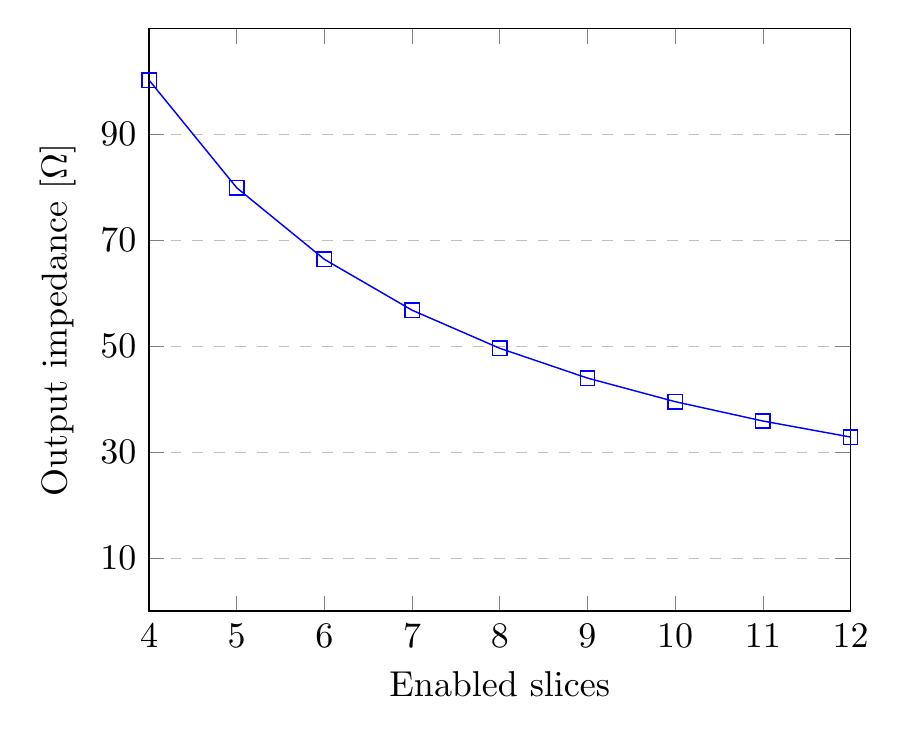
\begin{tikzpicture}[scale=1.3]
  \begin{axis}[
    %title={Output impedance tuning range},
    xlabel={Enabled slices},
    ylabel={Output impedance [$\Omega$]},
    xmin=4, xmax=12,
    ymin=0, ymax=110,
    xtick={4,5,6,7,8,9,10,11,12},
    ytick={10,30,50,70,90},
    ymajorgrids=true,
    grid style=dashed,
  ]

  \addplot[
    color=blue,
    mark=square,
    ]
    coordinates {
    (4,100.24)(5,79.92)(6,66.41)(7,56.81)(8,49.62)(9,44.00)(10,39.55)(11,35.90)(12,32.87)
    };

  \end{axis}
  \end{tikzpicture}
  \caption{Output impedance tuning range}
  \label{fig:imp_tuning_tx}
\end{figure}

